\documentclass[a4paper,12pt]{article}
\usepackage{iftex}
\ifPDFTeX
  \usepackage[T2A]{fontenc}
  \usepackage[utf8]{inputenc}
  \usepackage[russian]{babel}
  \usepackage{helvet}
  \renewcommand{\familydefault}{\sfdefault}
\else
  \usepackage{fontspec}
  \setmainfont{DejaVu Sans}
  \usepackage{polyglossia}
  \setdefaultlanguage{russian}
\fi

\usepackage{amsmath,amssymb,amsthm,mathtools}
\usepackage{icomma}
\usepackage[a4paper,margin=1.65cm,headheight=16pt]{geometry}
\usepackage{microtype}
\microtypesetup{expansion=false}
\usepackage{graphicx}
\usepackage{tikz}
\usetikzlibrary{positioning,arrows.meta,calc}
\usepackage{pgfplots}
\pgfplotsset{compat=1.18}
\usepackage{tabularx,booktabs,longtable}
\usepackage{enumitem}
\usepackage{hyperref}
\usepackage{parskip}
\usepackage{fancyhdr}
\usepackage{setspace}
\usepackage{xcolor}
\usepackage[most]{tcolorbox}
\usepackage{multicol}

\definecolor{accent}{HTML}{287F7A}
\definecolor{darkaccent}{HTML}{1C3151}
\definecolor{textgray}{HTML}{333333}
\definecolor{softteal}{HTML}{E4F3EF}
\definecolor{softcoral}{HTML}{FBE4DC}
\definecolor{coral}{HTML}{E77B5E}
\definecolor{softgold}{HTML}{F8EDCF}
\definecolor{softblue}{HTML}{E8EEF6}

\hypersetup{colorlinks=true,linkcolor=darkaccent,urlcolor=accent}
\setlist[itemize]{leftmargin=1.5em,itemsep=0.27em,topsep=0.35em}
\setlist[enumerate]{leftmargin=1.8em,itemsep=0.35em,topsep=0.35em}
\pagestyle{fancy}
\fancyhf{}
\lhead{Логарифмические неравенства}
\rhead{Тимофей Васильченко}
\cfoot{\thepage}
\renewcommand{\headrulewidth}{0.4pt}
\renewcommand{\today}{21 июля 2026 г.}
\onehalfspacing

\newtcolorbox{keybox}[1][]{enhanced,breakable,colback=softteal,colframe=accent,
  boxrule=0.7pt,arc=2.5mm,left=4mm,right=4mm,top=3mm,bottom=3mm,
  title=#1,fonttitle=\bfseries,coltitle=darkaccent}
\newtcolorbox{warnbox}[1][]{enhanced,breakable,colback=softcoral,colframe=coral,
  boxrule=0.7pt,arc=2.5mm,left=4mm,right=4mm,top=3mm,bottom=3mm,
  title=#1,fonttitle=\bfseries,coltitle=darkaccent}
\newtcolorbox{examplebox}[1][]{enhanced,breakable,colback=softblue,colframe=darkaccent,
  boxrule=0.7pt,arc=2.5mm,left=4mm,right=4mm,top=3mm,bottom=3mm,
  title=#1,fonttitle=\bfseries,coltitle=darkaccent}

\newcommand{\R}{\mathbb{R}}

\begin{document}

\begin{titlepage}
\centering
\vspace*{2.2cm}
{\color{accent}\Large\bfseries ЧЕК-ЛИСТ\par}
\vspace{0.45cm}
{\color{darkaccent}\fontsize{30}{35}\selectfont\bfseries
Логарифмические неравенства:\\
ОДЗ, монотонность и замена\par}
\vspace{0.85cm}
{\large Сравнение логарифмов, свойства, системы ограничений и типовые модели ЕГЭ\par}
\vfill
{\Large\bfseries Лёвин Артём Александрович\\[0.2cm]
эксклюзивно для Тимофея Васильченко\par}
\vspace{0.8cm}
{\large \today\par}
\vfill
\begin{tikzpicture}[remember picture,overlay]
  \draw[accent,line width=2.2pt] (-7,-1.2) .. controls (-4.7,1.15) and (-2.1,-2.1) .. (0.1,0.05)
    .. controls (2.25,2.05) and (4.85,-0.85) .. (7,0.8);
  \fill[accent!35] (-6.0,-0.32) circle (3pt);
  \fill[accent!60] (0.15,-0.12) circle (3pt);
  \fill[accent!85] (6.15,0.24) circle (3pt);
\end{tikzpicture}
\end{titlepage}

\section*{1. Главная идея}
\begin{keybox}[Логарифмическое неравенство решается в два слоя]
Сначала обеспечьте существование каждого логарифма, затем используйте монотонность
логарифмической функции. Итоговый ответ всегда является пересечением:
\[
\text{решение преобразованного неравенства}
\quad\cap\quad
\text{область допустимых значений}.
\]
\end{keybox}

\begin{center}
\begin{tikzpicture}[
  node distance=7mm and 8mm,
  >=Stealth,
  every node/.style={font=\small,align=center,rounded corners=2.5mm,minimum height=10mm}
]
\node[draw,fill=softgold,text width=3.0cm] (a) {Выписать ОДЗ};
\node[draw,fill=softteal,text width=3.2cm,right=of a] (b) {Определить основание};
\node[draw,fill=softblue,text width=3.2cm,right=of b] (c) {Преобразовать логарифмы};
\node[draw,fill=softcoral,text width=3.2cm,right=of c] (d) {Решить и пересечь};
\draw[->,thick,accent] (a)--(b);
\draw[->,thick,accent] (b)--(c);
\draw[->,thick,accent] (c)--(d);
\end{tikzpicture}
\end{center}

\section*{2. Область допустимых значений}
\begin{keybox}[Когда существует логарифм]
Выражение
\[
\log_a F(x)
\]
имеет смысл тогда и только тогда, когда
\[
a>0,\qquad a\ne1,\qquad F(x)>0.
\]
Если в задаче несколько логарифмов, положительным должен быть аргумент каждого из них.
\end{keybox}

\begin{warnbox}[ОДЗ записывается до преобразований]
Даже если после объединения логарифмов отдельный аргумент исчез из записи, исходное
условие его положительности сохраняется.
\end{warnbox}

\section*{3. Монотонность и сравнение логарифмов}
\begin{keybox}[Основание больше единицы]
Если $a>1$, функция $y=\log_a x$ возрастает:
\[
\log_a F(x)>\log_a G(x)
\Longleftrightarrow
\begin{cases}
F(x)>0,\\
G(x)>0,\\
F(x)>G(x).
\end{cases}
\]
Знак сравнения сохраняется.
\end{keybox}

\begin{keybox}[Основание между нулём и единицей]
Если $0<a<1$, функция $y=\log_a x$ убывает:
\[
\log_a F(x)>\log_a G(x)
\Longleftrightarrow
\begin{cases}
F(x)>0,\\
G(x)>0,\\
F(x)<G(x).
\end{cases}
\]
Знак сравнения меняется.
\end{keybox}

\begin{center}
\begin{tikzpicture}
\begin{axis}[
  width=13.2cm,height=6.8cm,
  axis lines=middle,
  xmin=-0.4,xmax=6.2,ymin=-4.2,ymax=3.2,
  samples=220,
  clip=false,
  grid=both,
  minor tick num=1,
  xlabel={$x$},ylabel={$y$},
  legend style={at={(0.98,0.04)},anchor=south east,draw=none,fill=white}
]
\addplot[domain=0.05:6,accent,very thick]{ln(x)/ln(2)};
\addlegendentry{$y=\log_2 x$ --- возрастает}
\addplot[domain=0.05:6,coral,very thick]{ln(x)/ln(0.5)};
\addlegendentry{$y=\log_{\frac12}x$ --- убывает}
\addplot[only marks,mark=*,darkaccent] coordinates {(1,0)};
\end{axis}
\end{tikzpicture}
\end{center}

\section*{4. Свойства, которые нужны в неравенствах}
При допустимых значениях аргументов:
\[
\log_a u+\log_a v=\log_a(uv),
\qquad
\log_a u-\log_a v=\log_a\frac{u}{v},
\]
\[
k\log_a u=\log_a(u^k),
\qquad
1=\log_a a.
\]

\begin{warnbox}[Условия применимости]
Для суммы нужны $u>0$ и $v>0$. Для разности также требуются $u>0$ и $v>0$.
Нельзя заменить два логарифма одним, забыв исходные ограничения.
\end{warnbox}

\section*{5. Универсальный алгоритм}
\begin{enumerate}
\item Выпишите условия положительности всех аргументов и ограничения на основание.
\item Приведите логарифмы к одному основанию, если это необходимо.
\item Перенесите числовые константы под знак логарифма: например, $1=\log_a a$.
\item Объедините сумму или разность логарифмов, сохраняя исходное ОДЗ.
\item Определите, больше основание единицы или меньше неё.
\item Сравните аргументы: сохраните или измените знак.
\item Решите полученное алгебраическое неравенство.
\item Пересеките решение с ОДЗ и проверьте границы.
\end{enumerate}

\section*{6. Разобранные примеры}

\begin{examplebox}[Пример 1. Константа рядом с логарифмом]
Решим
\[
1+\log_2 x>\log_2 5.
\]
ОДЗ: $x>0$. Представим единицу как $\log_2 2$:
\[
\log_2 2+\log_2 x>\log_2 5,
\]
\[
\log_2(2x)>\log_2 5.
\]
Основание $2>1$, поэтому знак сохраняется:
\[
2x>5,\qquad x>\frac52.
\]
Условие $x>0$ выполнено автоматически.
\[
\boxed{x\in\left(\frac52;+\infty\right)}.
\]
\end{examplebox}

\begin{examplebox}[Пример 2. ОДЗ и сравнение аргументов]
Решим
\[
\log_2(x^2-x-6)<\log_2(x-2).
\]
ОДЗ:
\[
\begin{cases}
x^2-x-6>0,\\
x-2>0.
\end{cases}
\]
Так как $x^2-x-6=(x-3)(x+2)$, получаем $x>3$.

Основание $2>1$, поэтому
\[
x^2-x-6<x-2,
\]
\[
x^2-2x-4<0.
\]
Корни: $x=1\pm\sqrt5$, следовательно,
\[
x\in(1-\sqrt5;1+\sqrt5).
\]
Пересекаем с $x>3$:
\[
\boxed{x\in(3;1+\sqrt5)}.
\]
\end{examplebox}

\begin{examplebox}[Пример 3. Замена переменной]
Решим
\[
(\log_2 x)^2-\log_2 x-6\le0.
\]
ОДЗ: $x>0$. Введём замену
\[
t=\log_2 x.
\]
Тогда
\[
t^2-t-6\le0,
\qquad
(t-3)(t+2)\le0,
\]
\[
-2\le t\le3.
\]
Возвращаемся к $x$. Основание $2>1$:
\[
-2\le\log_2 x\le3
\Longleftrightarrow
2^{-2}\le x\le2^3.
\]
\[
\boxed{x\in\left[\frac14;8\right]}.
\]
\end{examplebox}

\begin{examplebox}[Пример 4. Основание меньше единицы]
Решим
\[
\log_{\frac13}(x^2-3x-4)>
\log_{\frac13}(x-1)+\log_{\frac13}(x+1).
\]
ОДЗ:
\[
x^2-3x-4>0,\qquad x-1>0,\qquad x+1>0.
\]
Отсюда $x>4$. Объединяем правую часть:
\[
\log_{\frac13}(x^2-3x-4)>
\log_{\frac13}(x^2-1).
\]
Так как $0<\frac13<1$, знак меняется:
\[
x^2-3x-4<x^2-1,
\]
\[
x>-1.
\]
Пересечение с ОДЗ $x>4$:
\[
\boxed{x\in(4;+\infty)}.
\]
\end{examplebox}

\section*{7. Замена \(t=\log_a x\)}
\begin{keybox}[Когда замена особенно полезна]
Если в выражении повторяются
\[
(\log_a x)^2,\qquad \log_a x,\qquad \text{число},
\]
задача становится квадратным неравенством относительно $t=\log_a x$.
После решения по $t$ каждый промежуток нужно вернуть к $x$ с учётом монотонности основания.
\end{keybox}

\begin{warnbox}[Типичная ловушка]
Условие $x>0$ следует из самого логарифма. Оно не заменяет обратный переход:
границы для $t$ необходимо перевести в степени основания.
\end{warnbox}

\section*{8. Рабочая доска занятия}
\IfFileExists{../images/21.07.26-board.jpg}{
\begin{center}
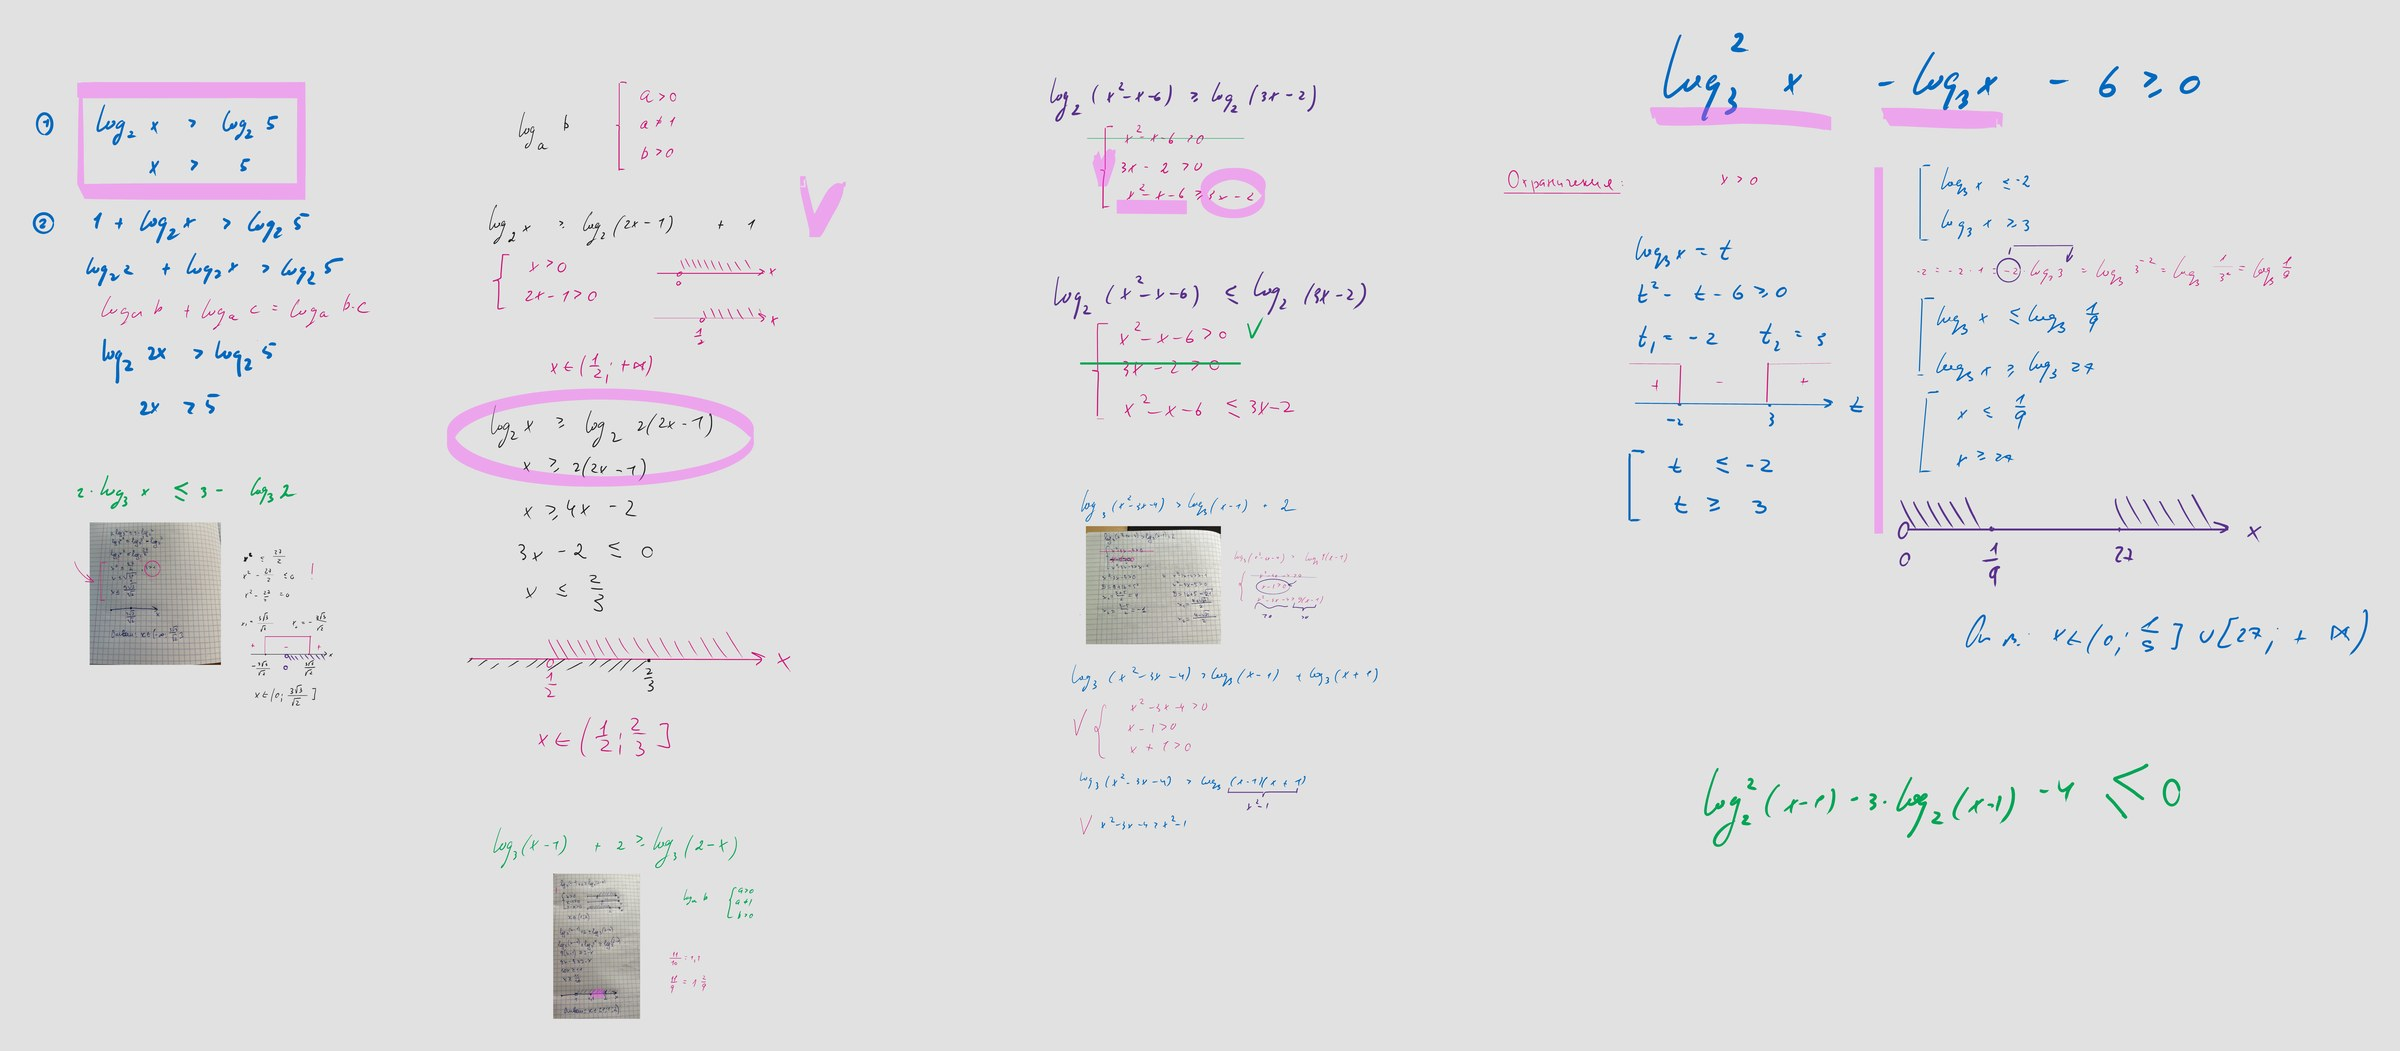
\includegraphics[width=\linewidth,height=0.48\textheight,keepaspectratio]{../images/21.07.26-board.jpg}
\end{center}
}{
\begin{center}
\begin{tabularx}{\linewidth}{@{}lX@{}}
\toprule
Этап & Содержание \\
\midrule
ОДЗ & аргументы логарифмов строго положительны \\
Основание & $a>1$ --- знак сохраняется; $0<a<1$ --- знак меняется \\
Свойства & сумма, разность, перенос константы под логарифм \\
Замена & $t=\log_a x$ и обязательный обратный переход \\
\bottomrule
\end{tabularx}
\end{center}
}

\section*{9. Типичные ошибки}
\begin{warnbox}
\begin{itemize}
\item Сравнить аргументы, не выписав их положительность.
\item Не изменить знак при основании $0<a<1$.
\item Записать $\log_a u+\log_a v=\log_a(u+v)$.
\item Объединить логарифмы и потерять ограничение одного из исходных аргументов.
\item Представить число единицей под логарифмом с неверным основанием.
\item После замены решить неравенство по $t$, но не вернуться к $x$.
\item Включить границу, на которой аргумент логарифма равен нулю.
\end{itemize}
\end{warnbox}

\section*{10. Итоговый чек-лист}
\begin{itemize}[label=$\square$]
\item Я проверяю $a>0$ и $a\ne1$.
\item Я требую положительности каждого аргумента.
\item Я знаю, когда знак сравнения сохраняется, а когда меняется.
\item Я умею представить $1$ как $\log_a a$.
\item Я объединяю сумму и разность логарифмов только при выполненном ОДЗ.
\item Я решаю алгебраическое неравенство после сравнения аргументов.
\item Я пересекаю полученный ответ с исходным ОДЗ.
\item Я применяю замену $t=\log_a x$ и выполняю обратный переход.
\item Я проверяю строгие и нестрогие границы.
\end{itemize}

\clearpage
\section*{Тренировочный блок}

\subsection*{Средний уровень}
\begin{enumerate}
\item Решите неравенство:
\[
\log_3 x>2.
\]

\item Решите неравенство:
\[
\log_{\frac12}(x-1)\ge-2.
\]

\item Решите неравенство:
\[
1+\log_2x\le\log_2 12.
\]
\end{enumerate}

\subsection*{Уровень выше среднего}
\begin{enumerate}[resume]
\item Решите:
\[
\log_5(x+4)>\log_5(2x-1).
\]

\item Решите:
\[
\log_{\frac13}(x+5)<\log_{\frac13}(2x-1).
\]

\item Решите:
\[
\log_2(x^2-5x+6)\ge\log_2(x-2).
\]

\item Решите:
\[
(\log_3x)^2-4\log_3x+3<0.
\]

\item Решите:
\[
\log_2(x-1)+\log_2(x+1)\le3.
\]

\item Решите:
\[
\log_{\frac12}(x^2-1)>\log_{\frac12}(3x-3).
\]
\end{enumerate}

\subsection*{Сложный уровень}
\begin{enumerate}[resume]
\item Решите:
\[
\log_{\frac13}(x^2-3x-4)>
\log_{\frac13}(x-1)+\log_{\frac13}(x+1).
\]
\end{enumerate}

\clearpage
\section*{Ответы}
\renewcommand{\arraystretch}{1.45}
\begin{longtable}{@{}cl@{}}
\toprule
№ & Ответ \\
\midrule
1 & $(9;+\infty)$ \\
2 & $(1;5]$ \\
3 & $(0;6]$ \\
4 & $\left(\dfrac12;5\right)$ \\
5 & $\left(\dfrac12;6\right)$ \\
6 & $[4;+\infty)$ \\
7 & $(3;27)$ \\
8 & $(1;3]$ \\
9 & $(1;2)$ \\
10 & $(4;+\infty)$ \\
\bottomrule
\end{longtable}

\end{document}
